\documentclass{jarticle}
\usepackage{amsmath,amssymb}
\usepackage{amsmath}
\usepackage[dvipdfmx]{graphicx}
\usepackage{here}
\usepackage{pifont}
\begin{document}
\title{BdGハミルトニアン}
\maketitle

\tableofcontents
\newpage
\section{導入}

ハミルトニアンは以下の式で表される。
\begin{align}
  H=\int\vec{\Psi}^\dagger(x,y)\tilde{H}\vec{\Psi}(x,y)dr
\end{align}

\begin{align}
\int{dr}=\int{dxdy}
\end{align}
\begin{align}
\vec{\Psi}=\begin{bmatrix}
\psi_{\uparrow} \\ 
\psi_{\downarrow} \\ 
\psi_{\uparrow}^\dagger \\ 
\psi_{\downarrow}^\dagger
\end{bmatrix} 
\end{align}
\begin{align}
\tilde{H}=
\begin{pmatrix}
	\hat{h}(r) & \hat{\Delta}(r) \\ 
	-\hat{\Delta}^{*}(r) & -\hat{h}^{*}(r)
\end{pmatrix} 
\end{align}
\begin{align}
\tilde{H}\in\mathbb{C}^4
\end{align}
\begin{align}
\hat{\Delta}(r),\tilde{h}(r)\in\mathbb{C}^{2\times 2}
\end{align}
\begin{align}
\tilde{h}=
\begin{bmatrix}
-\dfrac{\hbar^2}{2m}\nabla^2-\mu_F
\end{bmatrix}
\hat{\sigma}_0
\end{align}
\begin{flushright}
$\hat{\sigma}_0$: 単位行列
\end{flushright}
\begin{align}
\nabla^2=\partial x^2+\partial y^2
\end{align}
\begin{align}
\hat{\Delta}(r)=
\begin{cases}
$\rm(\hspace{.18em}i\hspace{.18em})\quad$\Delta_0(i\sigma_2)
& s-wave
\vspace*{1em}\\
$\rm(\hspace{.18em}ii\hspace{.18em})$\quad\Delta_0\dfrac{i\partial x}{k_F}\hat\sigma_1
&p_x-wave
\vspace*{1em}\\
$\rm(\hspace{.18em}iii\hspace{.18em})$\quad\Delta_0\dfrac{1}{k_F}(\partial x+i\partial y)\hat\sigma_1\
&p_x+ip_y
\end{cases}
\label{delta}
\end{align}
\begin{figure}[H]
	\centering
%	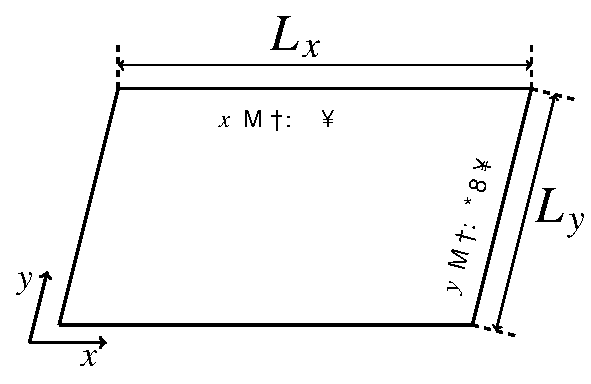
\includegraphics[scale=1]{./figure1.pdf}
	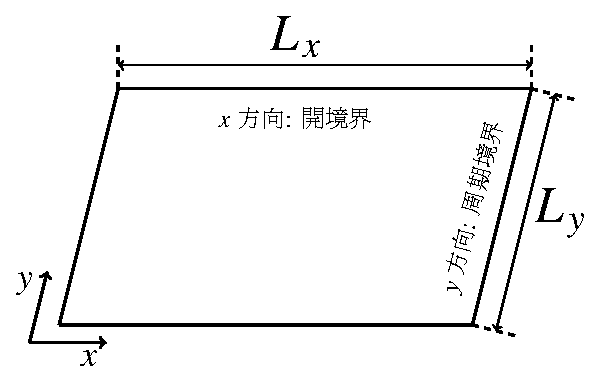
\includegraphics[scale=1]{./figure_fix.pdf}
	\caption{考える系}
	\label{system}
\end{figure}
図\ref{system}の系を考える。$y$方向には境界条件が課されている。
\begin{align}
 \vec{\Psi}=\dfrac{1}{\sqrt{l_y}}\displaystyle\sum_{k_y}\vec{\Psi}_{k_y}(x)e^{ik_yy}
\end{align}
%式\eqref{delta}
1.(i)の$\hat{\Delta}$を使う\\
\ding{"AC}$H$をフーリエ変換しましょう!$y$を波数に変換して一旦固定して$x$の関数として考えます。
\\ ヒント: (1)に(2)を代入しましょう。\\
\ding{"AD}離散化しましょう\\
\begin{align}
 H\rightarrow \tilde{H}
\end{align}
\begin{align}
  \tilde{H}=\vec{\Psi}\tilde{H}\vec{\Psi}
 \end{align}
 \begin{align}
  \vec{\Psi}=\begin{bmatrix}
  \psi_{1\uparrow} \\ 
  \psi_{1\downarrow} \\ 
  \psi_{1\uparrow}^\dagger \\ 
  \psi_{1\downarrow}^\dagger\\
  \psi_{2\uparrow} \\ 
  \psi_{2\downarrow} \\ 
  \vdots
 \end{bmatrix}
\end{align}
\begin{align}
\tilde{H}=
\begin{pmatrix}
\tilde{H} &  &  &  \\ 
& \tilde{H} &  &  \\ 
&  & \tilde{H} &  \\ 
&  &  & \ddots
\end{pmatrix} 
\end{align}
\begin{align}
\dfrac{\hbar^2}{2m}=t
\end{align}
とする。\\
\ding{"AE}差分近似しましょう\\
\begin{align}
\partial_x \psi_i\rightarrow?\\
\partial^2_x \psi_i\rightarrow?\\
\end{align}
刻み幅は1
\ding{"AF}$\tilde{H}$を対角化しましょう。数値計算\\
2(ii)の$\hat{\Delta}$を使う\\
\end{document}
